\documentclass[8pt,aspectratio=169]{beamer}
\usetheme{Madrid}
\usepackage{graphicx}
\usepackage{booktabs}
\usepackage{adjustbox}
\usepackage{multicol}
\usepackage{amsmath}
\usepackage{amssymb}
\usepackage{listings}
\usepackage{xcolor}

% Color definitions
\definecolor{mlblue}{RGB}{0,102,204}
\definecolor{mlpurple}{RGB}{51,51,178}
\definecolor{mllavender}{RGB}{173,173,224}
\definecolor{mllavender2}{RGB}{193,193,232}
\definecolor{mllavender3}{RGB}{204,204,235}
\definecolor{mllavender4}{RGB}{214,214,239}
\definecolor{mlorange}{RGB}{255, 127, 14}
\definecolor{mlgreen}{RGB}{44, 160, 44}
\definecolor{mlred}{RGB}{214, 39, 40}
\definecolor{mlgray}{RGB}{127, 127, 127}

% Additional colors for template compatibility
\definecolor{lightgray}{RGB}{240, 240, 240}
\definecolor{midgray}{RGB}{180, 180, 180}

% Solidity colors
\definecolor{solkeyword}{RGB}{0,102,153}
\definecolor{solstring}{RGB}{163,21,21}
\definecolor{solcomment}{RGB}{0,128,0}
\definecolor{solnumber}{RGB}{0,128,128}

% Solidity language definition
\lstdefinelanguage{Solidity}{
  keywords={pragma, solidity, contract, function, public, private, external, internal, view, pure, payable, returns, return, if, else, for, while, mapping, address, uint, uint256, int, string, bool, bytes, bytes32, event, emit, modifier, require, constructor, memory, storage, calldata, msg, sender, value, this, new, delete, true, false},
  keywordstyle=\color{solkeyword}\bfseries,
  sensitive=true,
  comment=[l]{//},
  morecomment=[s]{/*}{*/},
  commentstyle=\color{solcomment}\ttfamily,
  stringstyle=\color{solstring}\ttfamily,
  morestring=[b]',
  morestring=[b]"
}

% Apply custom colors to Madrid theme
\setbeamercolor{palette primary}{bg=mllavender3,fg=mlpurple}
\setbeamercolor{palette secondary}{bg=mllavender2,fg=mlpurple}
\setbeamercolor{palette tertiary}{bg=mllavender,fg=white}
\setbeamercolor{palette quaternary}{bg=mlpurple,fg=white}

\setbeamercolor{structure}{fg=mlpurple}
\setbeamercolor{section in toc}{fg=mlpurple}
\setbeamercolor{subsection in toc}{fg=mlblue}
\setbeamercolor{title}{fg=mlpurple}
\setbeamercolor{frametitle}{fg=mlpurple,bg=mllavender3}
\setbeamercolor{block title}{bg=mllavender2,fg=mlpurple}
\setbeamercolor{block body}{bg=mllavender4,fg=black}

% Remove navigation symbols
\setbeamertemplate{navigation symbols}{}

% Clean itemize/enumerate
\setbeamertemplate{itemize items}[circle]
\setbeamertemplate{enumerate items}[default]

% Reduce margins for more content space
\setbeamersize{text margin left=5mm,text margin right=5mm}

% Command for bottom annotation (Madrid-style)
\newcommand{\bottomnote}[1]{%
\vfill
\vspace{-2mm}
\textcolor{mllavender2}{\rule{\textwidth}{0.4pt}}
\vspace{1mm}
\footnotesize
\textbf{#1}
}

% TikZ and pgfplots packages
\usepackage{tikz}
\usepackage{pgfplots}
\pgfplotsset{compat=1.18}
\usetikzlibrary{arrows.meta, positioning, shapes.geometric, shapes.symbols, calc, decorations.pathmorphing, mindmap}

\title{Ethereum \& Smart Contracts: A Visual Introduction}
\subtitle{Standalone Mini-Lecture}
\author{Prof.~Dr.~Joerg Osterrieder}
\institute{University Lecture Series}
\date{\today}

\begin{document}

% ==================== FRAME 1: TITLE ====================
\begin{frame}[plain]
\vspace{2cm}
\begin{center}
{\Huge\color{mlpurple} Ethereum \& Smart Contracts}\\[0.4cm]
{\Large\color{mlblue} A Visual Introduction}\\[0.3cm]
{\normalsize Standalone Mini-Lecture}\\[0.3cm]
\textcolor{mlgray}{\rule{6cm}{0.4pt}}\\[0.3cm]
{\small\itshape ``Code is law -- until it's not''}\\[1.5cm]
{\normalsize Prof.~Dr.~Joerg Osterrieder}\\[0.2cm]
{\small University Lecture Series}\\[0.2cm]
{\small \today}
\end{center}
\end{frame}

% ==================== FRAME 2: THE PROGRAMMABLE MONEY PROBLEM (Comic Strip 1) ====================
\begin{frame}{The Programmable Money Problem}
\begin{center}
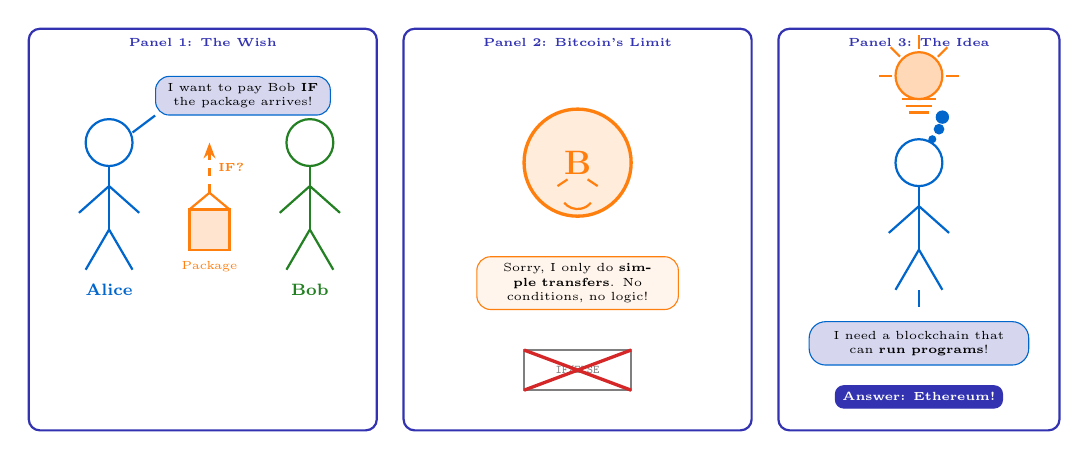
\begin{tikzpicture}[scale=0.85, every node/.style={transform shape}]

% --- Panel 1: Alice wants conditional payment ---
\draw[mlpurple, thick, rounded corners=4pt] (-7.2,-2.8) rectangle (-2.0,3.2);
\node[font=\tiny\bfseries, mlpurple] at (-4.6,3.0) {Panel 1: The Wish};

% Alice stick figure
\draw[mlblue, thick] (-6.0,1.5) circle (0.35);
\draw[mlblue, thick] (-6.0,1.15) -- (-6.0,0.2);
\draw[mlblue, thick] (-6.0,0.85) -- (-6.45,0.45);
\draw[mlblue, thick] (-6.0,0.85) -- (-5.55,0.45);
\draw[mlblue, thick] (-6.0,0.2) -- (-6.35,-0.4);
\draw[mlblue, thick] (-6.0,0.2) -- (-5.65,-0.4);
\node[font=\scriptsize\bfseries, mlblue] at (-6.0,-0.7) {Alice};

% Alice speech bubble
\node[draw=mlblue, fill=mllavender4, rounded corners=5pt, font=\tiny,
      text width=2.4cm, align=center, inner sep=3pt]
      (alice-bubble) at (-4.0,2.2) {I want to pay Bob \textbf{IF} the package arrives!};
\draw[mlblue, thick] (-5.65,1.65) -- (alice-bubble.south west);

% Bob stick figure
\draw[mlgreen!80!black, thick] (-3.0,1.5) circle (0.35);
\draw[mlgreen!80!black, thick] (-3.0,1.15) -- (-3.0,0.2);
\draw[mlgreen!80!black, thick] (-3.0,0.85) -- (-3.45,0.45);
\draw[mlgreen!80!black, thick] (-3.0,0.85) -- (-2.55,0.45);
\draw[mlgreen!80!black, thick] (-3.0,0.2) -- (-3.35,-0.4);
\draw[mlgreen!80!black, thick] (-3.0,0.2) -- (-2.65,-0.4);
\node[font=\scriptsize\bfseries, mlgreen!80!black] at (-3.0,-0.7) {Bob};

% Package icon between them
\draw[mlorange, thick, fill=mlorange!20] (-4.8,-0.1) rectangle (-4.2,0.5);
\draw[mlorange, thick] (-4.8,0.5) -- (-4.5,0.75) -- (-4.2,0.5);
\node[font=\tiny, mlorange] at (-4.5,-0.35) {Package};

% Conditional arrow
\draw[-{Stealth[length=2mm]}, mlorange, thick, dashed] (-4.5,0.75) -- (-4.5,1.5)
      node[midway, right, font=\tiny\bfseries, mlorange] {IF?};

% --- Panel 2: Bitcoin says no ---
\draw[mlpurple, thick, rounded corners=4pt] (-1.6,-2.8) rectangle (3.6,3.2);
\node[font=\tiny\bfseries, mlpurple] at (1.0,3.0) {Panel 2: Bitcoin's Limit};

% Bitcoin logo (simple circle with B)
\draw[mlorange, very thick, fill=mlorange!15] (1.0,1.2) circle (0.8);
\node[font=\Large\bfseries, mlorange] at (1.0,1.2) {B};

% Sad face on Bitcoin
\draw[mlorange, thick] (0.7,0.85) -- (0.85,0.95);
\draw[mlorange, thick] (1.3,0.85) -- (1.15,0.95);
\draw[mlorange, thick] (0.8,0.6) arc (220:320:0.26);

% Speech bubble from Bitcoin
\node[draw=mlorange, fill=mlorange!8, rounded corners=5pt, font=\tiny,
      text width=2.8cm, align=center, inner sep=3pt]
      at (1.0,-0.6) {Sorry, I only do \textbf{simple transfers}. No conditions, no logic!};

% Small script icon crossed out
\draw[mlgray, thick] (0.2,-1.6) rectangle (1.8,-2.2);
\node[font=\tiny, mlgray] at (1.0,-1.9) {\texttt{IF/ELSE}};
\draw[mlred, very thick] (0.2,-1.6) -- (1.8,-2.2);
\draw[mlred, very thick] (1.8,-1.6) -- (0.2,-2.2);

% --- Panel 3: Lightbulb moment ---
\draw[mlpurple, thick, rounded corners=4pt] (4.0,-2.8) rectangle (8.2,3.2);
\node[font=\tiny\bfseries, mlpurple] at (6.1,3.0) {Panel 3: The Idea};

% Alice thinking
\draw[mlblue, thick] (6.1,1.2) circle (0.35);
\draw[mlblue, thick] (6.1,0.85) -- (6.1,-0.1);
\draw[mlblue, thick] (6.1,0.55) -- (5.65,0.15);
\draw[mlblue, thick] (6.1,0.55) -- (6.55,0.15);
\draw[mlblue, thick] (6.1,-0.1) -- (5.75,-0.7);
\draw[mlblue, thick] (6.1,-0.1) -- (6.45,-0.7);

% Lightbulb
\draw[mlorange, thick, fill=mlorange!30] (6.1,2.5) circle (0.35);
\draw[mlorange, thick] (5.85,2.15) -- (6.35,2.15);
\draw[mlorange, thick] (5.9,2.05) -- (6.3,2.05);
\draw[mlorange, thick] (5.95,1.95) -- (6.25,1.95);
% Rays
\foreach \angle in {0,45,90,135,180} {
    \draw[mlorange, thick] ($(6.1,2.5)+(\angle:0.4)$) -- ($(6.1,2.5)+(\angle:0.6)$);
}

% Thought bubble chain
\fill[mlblue] (6.3,1.55) circle (0.06);
\fill[mlblue] (6.4,1.7) circle (0.08);
\fill[mlblue] (6.45,1.88) circle (0.1);

% Thought content
\node[draw=mlblue, fill=mllavender4, rounded corners=6pt, font=\tiny,
      text width=3.0cm, align=center, inner sep=4pt]
      at (6.1,-1.5) {I need a blockchain that can \textbf{run programs}!};
\draw[mlblue, thick] (6.1,-0.7) -- (6.1,-0.95);

% Arrow to answer
\node[draw=mlpurple, fill=mlpurple, text=white, rounded corners=3pt, font=\tiny\bfseries,
      inner sep=3pt] at (6.1,-2.3) {Answer: Ethereum!};

\end{tikzpicture}
\end{center}

\bottomnote{Key insight: Bitcoin's scripting language is intentionally limited. Ethereum was designed from the ground up as a programmable blockchain.}
\end{frame}

% ==================== FRAME 3: ENTER ETHEREUM (Comic Strip 2) ====================
\begin{frame}{Enter Ethereum: The World Computer}
\begin{center}
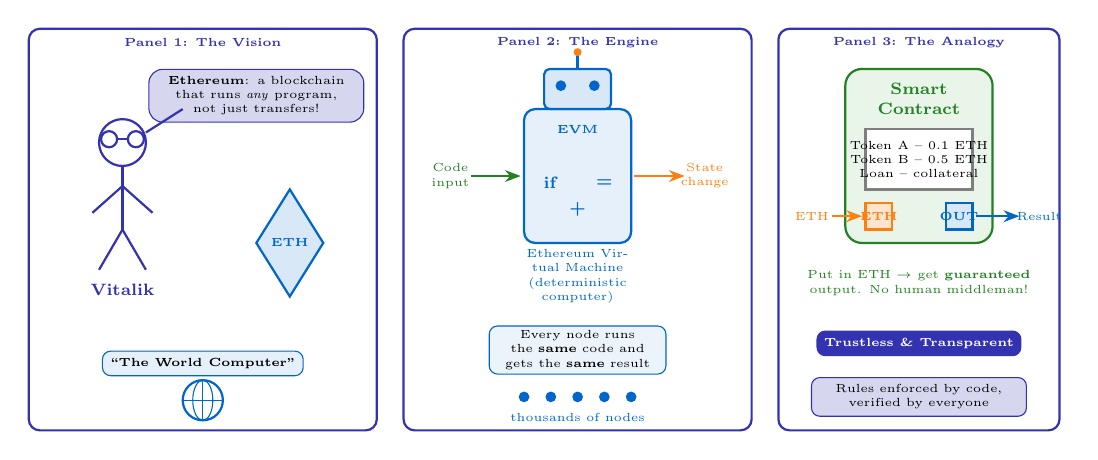
\begin{tikzpicture}[scale=0.85, every node/.style={transform shape}]

% --- Panel 1: Vitalik introduces Ethereum ---
\draw[mlpurple, thick, rounded corners=4pt] (-7.2,-2.8) rectangle (-2.0,3.2);
\node[font=\tiny\bfseries, mlpurple] at (-4.6,3.0) {Panel 1: The Vision};

% Vitalik stick figure (with glasses)
\draw[mlpurple, thick] (-5.8,1.5) circle (0.35);
\draw[mlpurple, thick] (-5.8,1.15) -- (-5.8,0.2);
\draw[mlpurple, thick] (-5.8,0.85) -- (-6.25,0.45);
\draw[mlpurple, thick] (-5.8,0.85) -- (-5.35,0.45);
\draw[mlpurple, thick] (-5.8,0.2) -- (-6.15,-0.4);
\draw[mlpurple, thick] (-5.8,0.2) -- (-5.45,-0.4);
% Glasses
\draw[mlpurple, thick] (-6.0,1.55) circle (0.12);
\draw[mlpurple, thick] (-5.6,1.55) circle (0.12);
\draw[mlpurple, thick] (-5.88,1.55) -- (-5.72,1.55);
\node[font=\scriptsize\bfseries, mlpurple] at (-5.8,-0.7) {Vitalik};

% Speech bubble
\node[draw=mlpurple, fill=mllavender4, rounded corners=5pt, font=\tiny,
      text width=3.0cm, align=center, inner sep=3pt]
      at (-3.8,2.2) {\textbf{Ethereum}: a blockchain that runs \emph{any} program, not just transfers!};
\draw[mlpurple, thick] (-5.45,1.65) -- (-4.9,2.0);

% Ethereum diamond logo
\draw[mlblue, thick, fill=mlblue!15] (-3.8,0.0) -- (-3.3,0.8) -- (-2.8,0.0) -- (-3.3,-0.8) -- cycle;
\node[font=\tiny\bfseries, mlblue] at (-3.3,0.0) {ETH};

% World Computer label
\node[draw=mlblue, fill=mlblue!10, rounded corners=3pt, font=\tiny\bfseries,
      inner sep=3pt] at (-4.6,-1.8) {``The World Computer''};

% Globe icon
\draw[mlblue, thick] (-4.6,-2.35) circle (0.3);
\draw[mlblue, thin] (-4.9,-2.35) -- (-4.3,-2.35);
\draw[mlblue, thin] (-4.6,-2.65) -- (-4.6,-2.05);
\draw[mlblue, thin] (-4.6,-2.35) ellipse (0.15 and 0.3);

% --- Panel 2: The EVM as a robot ---
\draw[mlpurple, thick, rounded corners=4pt] (-1.6,-2.8) rectangle (3.6,3.2);
\node[font=\tiny\bfseries, mlpurple] at (1.0,3.0) {Panel 2: The Engine};

% EVM Robot body
\draw[mlblue, thick, fill=mlblue!10, rounded corners=4pt] (0.2,0.0) rectangle (1.8,2.0);
\node[font=\tiny\bfseries, mlblue] at (1.0,1.7) {EVM};

% Robot head
\draw[mlblue, thick, fill=mlblue!15, rounded corners=2pt] (0.5,2.0) rectangle (1.5,2.6);
% Eyes
\fill[mlblue] (0.75,2.35) circle (0.08);
\fill[mlblue] (1.25,2.35) circle (0.08);
% Antenna
\draw[mlblue, thick] (1.0,2.6) -- (1.0,2.85);
\fill[mlorange] (1.0,2.85) circle (0.06);

% Code going in (left)
\draw[-{Stealth[length=2mm]}, mlgreen!80!black, thick] (-0.6,1.0) -- (0.15,1.0);
\node[font=\tiny, mlgreen!80!black, align=center] at (-0.9,1.0) {Code\\input};

% Result coming out (right)
\draw[-{Stealth[length=2mm]}, mlorange, thick] (1.85,1.0) -- (2.6,1.0);
\node[font=\tiny, mlorange, align=center] at (2.9,1.0) {State\\change};

% Gears inside robot
\node[font=\scriptsize, mlblue] at (0.6,0.9) {\textbf{if}};
\node[font=\scriptsize, mlblue] at (1.0,0.5) {\textbf{+}};
\node[font=\scriptsize, mlblue] at (1.4,0.9) {\textbf{=}};

% Label
\node[font=\tiny, mlblue, text width=2.5cm, align=center] at (1.0,-0.5) {Ethereum Virtual Machine\\(deterministic computer)};

% Every node runs it
\node[draw=mlblue, fill=mlblue!8, rounded corners=3pt, font=\tiny,
      inner sep=2pt, text width=2.5cm, align=center] at (1.0,-1.6) {Every node runs the \textbf{same} code and gets the \textbf{same} result};

% Small nodes
\foreach \x in {0.2,0.6,1.0,1.4,1.8} {
    \fill[mlblue] (\x,-2.3) circle (0.08);
}
\node[font=\tiny, mlblue] at (1.0,-2.6) {thousands of nodes};

% --- Panel 3: Vending machine ---
\draw[mlpurple, thick, rounded corners=4pt] (4.0,-2.8) rectangle (8.2,3.2);
\node[font=\tiny\bfseries, mlpurple] at (6.1,3.0) {Panel 3: The Analogy};

% Vending machine body
\draw[mlgreen!80!black, thick, fill=mlgreen!10, rounded corners=6pt]
     (5.0,0.0) rectangle (7.2,2.6);
\node[font=\scriptsize\bfseries, mlgreen!80!black] at (6.1,2.3) {Smart};
\node[font=\scriptsize\bfseries, mlgreen!80!black] at (6.1,2.0) {Contract};

% Display window with items
\draw[mlgray, thick, fill=white] (5.3,0.8) rectangle (6.9,1.7);
\node[font=\tiny, align=center] at (6.1,1.25) {Token A -- 0.1 ETH\\Token B -- 0.5 ETH\\Loan -- collateral};

% Coin slot
\draw[mlorange, thick, fill=mlorange!20] (5.3,0.2) rectangle (5.7,0.6);
\node[font=\tiny\bfseries, mlorange] at (5.5,0.4) {ETH};

% Output slot
\draw[mlblue, thick, fill=mlblue!15] (6.5,0.2) rectangle (6.9,0.6);
\node[font=\tiny\bfseries, mlblue] at (6.7,0.4) {OUT};

% Arrow: ETH in
\draw[-{Stealth[length=2mm]}, mlorange, thick] (4.8,0.4) -- (5.25,0.4);
\node[font=\tiny, mlorange] at (4.5,0.4) {ETH};

% Arrow: output out
\draw[-{Stealth[length=2mm]}, mlblue, thick] (6.95,0.4) -- (7.6,0.4);
\node[font=\tiny, mlblue, align=center] at (7.9,0.4) {Result};

% Label
\node[font=\tiny, mlgreen!80!black, text width=3.5cm, align=center]
      at (6.1,-0.6) {Put in ETH $\to$ get \textbf{guaranteed} output. No human middleman!};

% Key guarantee
\node[draw=mlpurple, fill=mlpurple, text=white, rounded corners=3pt, font=\tiny\bfseries,
      inner sep=3pt] at (6.1,-1.5) {Trustless \& Transparent};

% Bottom note
\node[draw=mlpurple, fill=mllavender4, rounded corners=3pt, font=\tiny,
      inner sep=3pt, text width=3.0cm, align=center] at (6.1,-2.3)
      {Rules enforced by code,\\verified by everyone};

\end{tikzpicture}
\end{center}

\bottomnote{Key insight: Ethereum extends blockchain from a payment ledger to a general-purpose computation platform --- the ``world computer.''}
\end{frame}

% ==================== FRAME 4: BITCOIN VS ETHEREUM ====================
\begin{frame}{Bitcoin vs Ethereum: Side-by-Side}
\vspace{-2mm}
\begin{center}
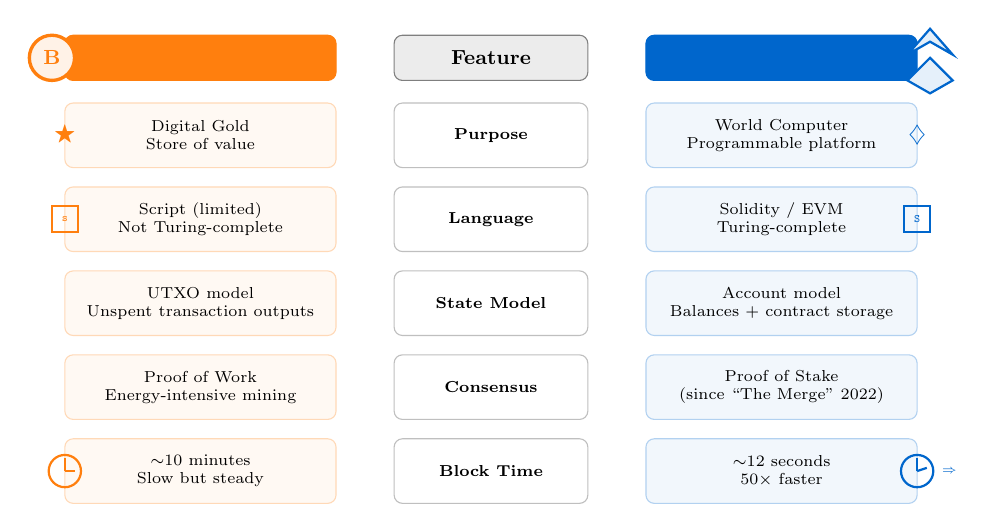
\begin{tikzpicture}[scale=0.82, every node/.style={transform shape}]

% Header row
\node[draw=mlgray, fill=mlgray!15, rounded corners=3pt, minimum width=3.0cm,
      minimum height=0.7cm, font=\small\bfseries] at (0,3.5) {Feature};
\node[draw=mlorange, fill=mlorange!15, rounded corners=3pt, minimum width=4.2cm,
      minimum height=0.7cm, font=\small\bfseries, mlorange] at (-4.5,3.5) {Bitcoin};
\node[draw=mlblue, fill=mlblue!15, rounded corners=3pt, minimum width=4.2cm,
      minimum height=0.7cm, font=\small\bfseries, mlblue] at (4.5,3.5) {Ethereum};

% Bitcoin logo
\draw[mlorange, very thick, fill=mlorange!10] (-6.8,3.5) circle (0.35);
\node[font=\small\bfseries, mlorange] at (-6.8,3.5) {B};

% Ethereum logo
\draw[mlblue, thick, fill=mlblue!10] (6.8,3.5) -- (7.15,3.15) -- (6.8,2.95) -- (6.45,3.15) -- cycle;
\draw[mlblue, thick, fill=mlblue!10] (6.8,3.95) -- (7.15,3.55) -- (6.8,3.75) -- (6.45,3.55) -- cycle;

% Row definitions: Feature / Bitcoin / Ethereum
% Row 1: Purpose
\node[draw=mlgray!50, fill=white, rounded corners=3pt, minimum width=3.0cm,
      minimum height=1.0cm, font=\scriptsize\bfseries, align=center] at (0,2.3) {Purpose};
\node[draw=mlorange!30, fill=mlorange!5, rounded corners=3pt, minimum width=4.2cm,
      minimum height=1.0cm, font=\scriptsize, align=center] at (-4.5,2.3) {Digital Gold\\Store of value};
\node[draw=mlblue!30, fill=mlblue!5, rounded corners=3pt, minimum width=4.2cm,
      minimum height=1.0cm, font=\scriptsize, align=center] at (4.5,2.3) {World Computer\\Programmable platform};

% Icon for row 1
\node[font=\normalsize, mlorange] at (-6.6,2.3) {$\bigstar$};
\node[font=\normalsize, mlblue] at (6.6,2.3) {$\diamondsuit$};

% Row 2: Language
\node[draw=mlgray!50, fill=white, rounded corners=3pt, minimum width=3.0cm,
      minimum height=1.0cm, font=\scriptsize\bfseries, align=center] at (0,1.0) {Language};
\node[draw=mlorange!30, fill=mlorange!5, rounded corners=3pt, minimum width=4.2cm,
      minimum height=1.0cm, font=\scriptsize, align=center] at (-4.5,1.0) {Script (limited)\\Not Turing-complete};
\node[draw=mlblue!30, fill=mlblue!5, rounded corners=3pt, minimum width=4.2cm,
      minimum height=1.0cm, font=\scriptsize, align=center] at (4.5,1.0) {Solidity / EVM\\Turing-complete};

% Icon for row 2
\draw[mlorange, thick] (-6.8,0.8) rectangle (-6.4,1.2);
\node[font=\tiny, mlorange] at (-6.6,1.0) {\texttt{s}};
\draw[mlblue, thick] (6.4,0.8) rectangle (6.8,1.2);
\node[font=\tiny, mlblue] at (6.6,1.0) {\texttt{S}};

% Row 3: State Model
\node[draw=mlgray!50, fill=white, rounded corners=3pt, minimum width=3.0cm,
      minimum height=1.0cm, font=\scriptsize\bfseries, align=center] at (0,-0.3) {State Model};
\node[draw=mlorange!30, fill=mlorange!5, rounded corners=3pt, minimum width=4.2cm,
      minimum height=1.0cm, font=\scriptsize, align=center] at (-4.5,-0.3) {UTXO model\\Unspent transaction outputs};
\node[draw=mlblue!30, fill=mlblue!5, rounded corners=3pt, minimum width=4.2cm,
      minimum height=1.0cm, font=\scriptsize, align=center] at (4.5,-0.3) {Account model\\Balances + contract storage};

% Row 4: Consensus
\node[draw=mlgray!50, fill=white, rounded corners=3pt, minimum width=3.0cm,
      minimum height=1.0cm, font=\scriptsize\bfseries, align=center] at (0,-1.6) {Consensus};
\node[draw=mlorange!30, fill=mlorange!5, rounded corners=3pt, minimum width=4.2cm,
      minimum height=1.0cm, font=\scriptsize, align=center] at (-4.5,-1.6) {Proof of Work\\Energy-intensive mining};
\node[draw=mlblue!30, fill=mlblue!5, rounded corners=3pt, minimum width=4.2cm,
      minimum height=1.0cm, font=\scriptsize, align=center] at (4.5,-1.6) {Proof of Stake\\(since ``The Merge'' 2022)};

% Row 5: Block Time
\node[draw=mlgray!50, fill=white, rounded corners=3pt, minimum width=3.0cm,
      minimum height=1.0cm, font=\scriptsize\bfseries, align=center] at (0,-2.9) {Block Time};
\node[draw=mlorange!30, fill=mlorange!5, rounded corners=3pt, minimum width=4.2cm,
      minimum height=1.0cm, font=\scriptsize, align=center] at (-4.5,-2.9) {$\sim$10 minutes\\Slow but steady};
\node[draw=mlblue!30, fill=mlblue!5, rounded corners=3pt, minimum width=4.2cm,
      minimum height=1.0cm, font=\scriptsize, align=center] at (4.5,-2.9) {$\sim$12 seconds\\50$\times$ faster};

% Clock icons
\draw[mlorange, thick] (-6.6,-2.9) circle (0.25);
\draw[mlorange, thick] (-6.6,-2.9) -- (-6.6,-2.7);
\draw[mlorange, thick] (-6.6,-2.9) -- (-6.45,-2.9);

\draw[mlblue, thick] (6.6,-2.9) circle (0.25);
\draw[mlblue, thick] (6.6,-2.9) -- (6.6,-2.7);
\draw[mlblue, thick] (6.6,-2.9) -- (6.75,-2.85);
% Lightning bolt for speed
\node[font=\tiny\bfseries, mlblue] at (7.1,-2.9) {$\!\Rightarrow\!$};

\end{tikzpicture}
\end{center}

\bottomnote{Key insight: Bitcoin optimizes for security and simplicity. Ethereum trades some simplicity for programmability --- different goals, different designs.}
\end{frame}

% ==================== FRAME 5: HOW GAS WORKS ====================
\begin{frame}{How Gas Works: Fueling the World Computer}
\vspace{-2mm}
\begin{center}
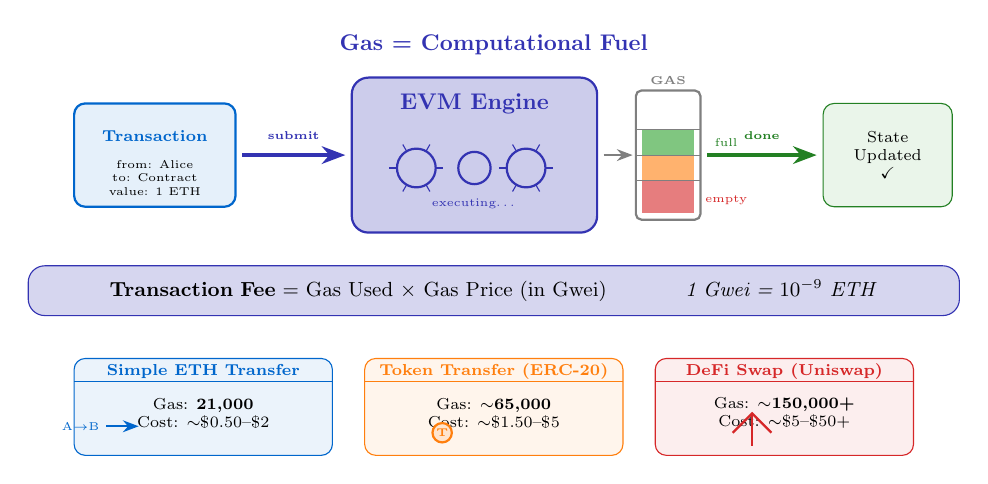
\begin{tikzpicture}[scale=0.82, every node/.style={transform shape}]

% === Car/Fuel Analogy (top) ===
\node[font=\normalsize\bfseries, mlpurple] at (0,3.5) {Gas = Computational Fuel};

% Transaction (car)
\draw[mlblue, thick, fill=mlblue!10, rounded corners=4pt] (-6.5,1.0) rectangle (-4.0,2.6);
\node[font=\scriptsize\bfseries, mlblue, align=center] at (-5.25,2.1) {Transaction};
\node[font=\tiny, align=center] at (-5.25,1.45) {from: Alice\\to: Contract\\value: 1 ETH};

% Arrow to EVM engine
\draw[-{Stealth[length=3mm]}, mlpurple, very thick] (-3.9,1.8) -- (-2.3,1.8);
\node[font=\tiny\bfseries, mlpurple] at (-3.1,2.1) {submit};

% EVM Engine block
\draw[mlpurple, thick, fill=mllavender3, rounded corners=6pt] (-2.2,0.6) rectangle (1.6,3.0);
\node[font=\normalsize\bfseries, mlpurple] at (-0.3,2.6) {EVM Engine};

% Gears inside
\draw[mlpurple, thick] (-1.2,1.6) circle (0.3);
\draw[mlpurple, thick] (-0.3,1.6) circle (0.25);
\draw[mlpurple, thick] (0.5,1.6) circle (0.3);
% Gear teeth (simplified lines)
\foreach \angle in {0,60,120,180,240,300} {
    \draw[mlpurple, thin] ($(-1.2,1.6)+(\angle:0.3)$) -- ($(-1.2,1.6)+(\angle:0.42)$);
    \draw[mlpurple, thin] ($(0.5,1.6)+(\angle:0.3)$) -- ($(0.5,1.6)+(\angle:0.42)$);
}
\node[font=\tiny, mlpurple] at (-0.3,1.05) {executing\ldots};

% Gas gauge (fuel draining)
\draw[mlgray, thick, rounded corners=2pt] (2.2,0.8) rectangle (3.2,2.8);
\node[font=\tiny\bfseries, mlgray] at (2.7,2.95) {GAS};
% Fuel level (partially drained)
\fill[mlred!60] (2.3,0.9) rectangle (3.1,1.4);
\fill[mlorange!60] (2.3,1.4) rectangle (3.1,1.8);
\fill[mlgreen!60] (2.3,1.8) rectangle (3.1,2.2);
% Drain line
\draw[mlgray, thin] (2.2,2.2) -- (3.2,2.2);
\draw[mlgray, thin] (2.2,1.8) -- (3.2,1.8);
\draw[mlgray, thin] (2.2,1.4) -- (3.2,1.4);
% Labels
\node[font=\tiny, mlgreen!80!black] at (3.6,2.0) {full};
\node[font=\tiny, mlred] at (3.6,1.1) {empty};

% Arrow from EVM to gauge
\draw[-{Stealth[length=2mm]}, mlgray, thick] (1.7,1.8) -- (2.15,1.8);

% Result arrow
\draw[-{Stealth[length=3mm]}, mlgreen!80!black, very thick] (3.3,1.8) -- (5.0,1.8);
\node[font=\tiny\bfseries, mlgreen!80!black] at (4.15,2.1) {done};

% Result
\node[draw=mlgreen!80!black, fill=mlgreen!10, rounded corners=4pt, minimum width=2.0cm,
      minimum height=1.6cm, font=\scriptsize, align=center] at (6.1,1.8)
      {State\\Updated\\$\checkmark$};

% === Formula Box (middle) ===
\node[draw=mlpurple, fill=mllavender4, rounded corners=6pt, inner sep=6pt,
      font=\small, text width=14cm, align=center]
      at (0,-0.3) {%
\textbf{Transaction Fee} = Gas Used $\times$ Gas Price (in Gwei)
\hspace{1cm}
\textit{1 Gwei = $10^{-9}$ ETH}};

% === Gas examples (bottom) ===
% Simple transfer
\node[draw=mlblue, fill=mlblue!8, rounded corners=4pt, minimum width=4.0cm,
      minimum height=1.5cm, inner sep=4pt] at (-4.5,-2.1) {};
\node[font=\scriptsize\bfseries, mlblue] at (-4.5,-1.55) {Simple ETH Transfer};
\draw[mlblue, thin] (-6.5,-1.7) -- (-2.5,-1.7);
\node[font=\scriptsize, align=center] at (-4.5,-2.2) {Gas: \textbf{21,000}\\Cost: $\sim$\$0.50--\$2};
% Small icon
\draw[-{Stealth[length=2mm]}, mlblue, thick] (-6.0,-2.4) -- (-5.5,-2.4);
\node[font=\tiny, mlblue] at (-6.4,-2.4) {A$\to$B};

% Contract call
\node[draw=mlorange, fill=mlorange!8, rounded corners=4pt, minimum width=4.0cm,
      minimum height=1.5cm, inner sep=4pt] at (0,-2.1) {};
\node[font=\scriptsize\bfseries, mlorange] at (0,-1.55) {Token Transfer (ERC-20)};
\draw[mlorange, thin] (-2.0,-1.7) -- (2.0,-1.7);
\node[font=\scriptsize, align=center] at (0,-2.2) {Gas: $\sim$\textbf{65,000}\\Cost: $\sim$\$1.50--\$5};
% Small icon
\draw[mlorange, thick, fill=mlorange!20] (-0.8,-2.5) circle (0.15);
\node[font=\tiny\bfseries, mlorange] at (-0.8,-2.5) {T};

% Complex DeFi
\node[draw=mlred, fill=mlred!8, rounded corners=4pt, minimum width=4.0cm,
      minimum height=1.5cm, inner sep=4pt] at (4.5,-2.1) {};
\node[font=\scriptsize\bfseries, mlred] at (4.5,-1.55) {DeFi Swap (Uniswap)};
\draw[mlred, thin] (2.5,-1.7) -- (6.5,-1.7);
\node[font=\scriptsize, align=center] at (4.5,-2.2) {Gas: $\sim$\textbf{150,000+}\\Cost: $\sim$\$5--\$50+};
% Small icon
\draw[mlred, thick] (3.7,-2.5) -- (4.0,-2.2) -- (4.3,-2.5);
\draw[mlred, thick] (4.0,-2.2) -- (4.0,-2.7);

\end{tikzpicture}
\end{center}

\bottomnote{Key insight: Gas prevents spam and infinite loops. Users pay for computation; validators earn fees for processing. EIP-1559 (2021) added a base fee burn mechanism.}
\end{frame}

% ==================== FRAME 6: SMART CONTRACT LIFECYCLE ====================
\begin{frame}{Smart Contract Lifecycle}
\vspace{-1mm}
\begin{center}
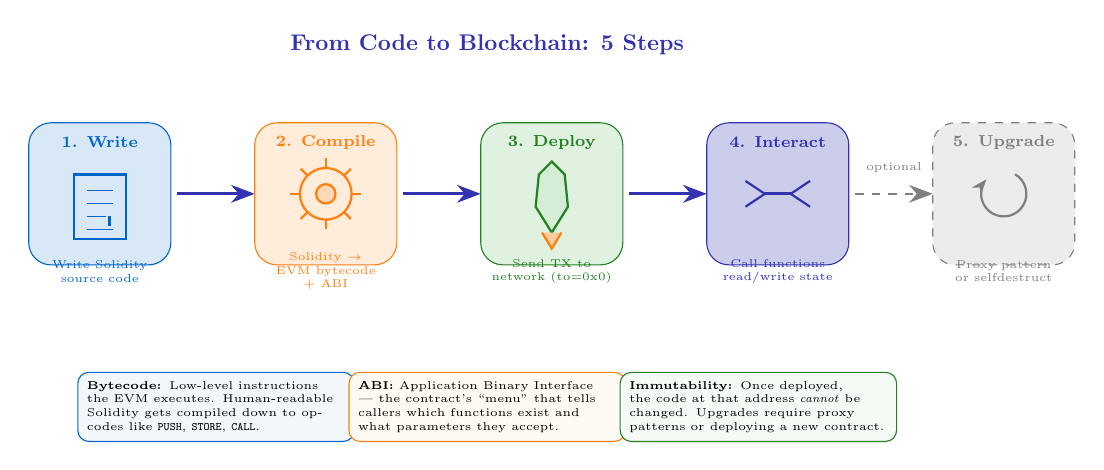
\begin{tikzpicture}[scale=0.82, every node/.style={transform shape}]

% Title
\node[font=\normalsize\bfseries, mlpurple] at (0,3.8) {From Code to Blockchain: 5 Steps};

% === Step 1: Write ===
\node[draw=mlblue, fill=mlblue!15, rounded corners=8pt, minimum width=2.2cm,
      minimum height=2.2cm, inner sep=3pt] (write) at (-6.0,1.5) {};
\node[font=\scriptsize\bfseries, mlblue] at (-6.0,2.3) {1. Write};

% Code icon (document with lines)
\draw[mlblue, thick] (-6.4,0.8) rectangle (-5.6,1.8);
\draw[mlblue, thin] (-6.2,1.55) -- (-5.8,1.55);
\draw[mlblue, thin] (-6.2,1.35) -- (-5.8,1.35);
\draw[mlblue, thin] (-6.2,1.15) -- (-5.9,1.15);
\draw[mlblue, thin] (-6.2,0.95) -- (-5.8,0.95);
% Cursor
\draw[mlblue, thick] (-5.85,1.15) -- (-5.85,1.0);

\node[font=\tiny, mlblue, text width=2.0cm, align=center] at (-6.0,0.3)
     {Write Solidity\\source code};

% Arrow 1->2
\draw[-{Stealth[length=3mm]}, mlpurple, very thick] (-4.8,1.5) -- (-3.6,1.5);

% === Step 2: Compile ===
\node[draw=mlorange, fill=mlorange!15, rounded corners=8pt, minimum width=2.2cm,
      minimum height=2.2cm, inner sep=3pt] (compile) at (-2.5,1.5) {};
\node[font=\scriptsize\bfseries, mlorange] at (-2.5,2.3) {2. Compile};

% Gear icon
\draw[mlorange, thick] (-2.5,1.5) circle (0.4);
\foreach \angle in {0,45,90,135,180,225,270,315} {
    \draw[mlorange, thick] ($(-2.5,1.5)+(\angle:0.4)$) -- ($(-2.5,1.5)+(\angle:0.55)$);
}
\draw[mlorange, thick, fill=mlorange!30] (-2.5,1.5) circle (0.15);

\node[font=\tiny, mlorange, text width=2.0cm, align=center] at (-2.5,0.3)
     {Solidity $\to$\\EVM bytecode\\+ ABI};

% Arrow 2->3
\draw[-{Stealth[length=3mm]}, mlpurple, very thick] (-1.3,1.5) -- (-0.1,1.5);

% === Step 3: Deploy ===
\node[draw=mlgreen!80!black, fill=mlgreen!15, rounded corners=8pt, minimum width=2.2cm,
      minimum height=2.2cm, inner sep=3pt] (deploy) at (1.0,1.5) {};
\node[font=\scriptsize\bfseries, mlgreen!80!black] at (1.0,2.3) {3. Deploy};

% Rocket icon
\draw[mlgreen!80!black, thick, fill=mlgreen!20] (1.0,0.9) -- (0.75,1.3) -- (0.8,1.8) --
     (1.0,2.0) -- (1.2,1.8) -- (1.25,1.3) -- cycle;
% Flame
\draw[mlorange, thick, fill=mlorange!40] (0.85,0.9) -- (1.0,0.65) -- (1.15,0.9);

\node[font=\tiny, mlgreen!80!black, text width=2.0cm, align=center] at (1.0,0.3)
     {Send TX to\\network (to=0x0)};

% Arrow 3->4
\draw[-{Stealth[length=3mm]}, mlpurple, very thick] (2.2,1.5) -- (3.4,1.5);

% === Step 4: Interact ===
\node[draw=mlpurple, fill=mllavender3, rounded corners=8pt, minimum width=2.2cm,
      minimum height=2.2cm, inner sep=3pt] (interact) at (4.5,1.5) {};
\node[font=\scriptsize\bfseries, mlpurple] at (4.5,2.3) {4. Interact};

% Handshake icon (two hands)
\draw[mlpurple, thick] (4.0,1.3) -- (4.3,1.5) -- (4.0,1.7);
\draw[mlpurple, thick] (5.0,1.3) -- (4.7,1.5) -- (5.0,1.7);
\draw[mlpurple, very thick] (4.3,1.5) -- (4.7,1.5);

\node[font=\tiny, mlpurple, text width=2.0cm, align=center] at (4.5,0.3)
     {Call functions\\read/write state};

% Arrow 4->5 (dashed)
\draw[-{Stealth[length=3mm]}, mlgray, thick, dashed] (5.7,1.5) -- (6.9,1.5);
\node[font=\tiny, mlgray] at (6.3,1.9) {optional};

% === Step 5: Upgrade/Destroy ===
\node[draw=mlgray, fill=mlgray!15, rounded corners=8pt, minimum width=2.2cm,
      minimum height=2.2cm, inner sep=3pt, dashed] (upgrade) at (8.0,1.5) {};
\node[font=\scriptsize\bfseries, mlgray] at (8.0,2.3) {5. Upgrade};

% Cycle/refresh icon
\draw[mlgray, thick, -{Stealth[length=2mm]}] (8.0,1.5) ++(60:0.35) arc (60:-220:0.35);

\node[font=\tiny, mlgray, text width=2.0cm, align=center] at (8.0,0.3)
     {Proxy pattern\\or selfdestruct};

% === Bottom detail boxes ===
\node[draw=mlblue, fill=mlblue!5, rounded corners=4pt, font=\tiny,
      inner sep=4pt, text width=4.0cm, align=left] at (-4.2,-1.8)
     {\textbf{Bytecode:} Low-level instructions the EVM executes.
      Human-readable Solidity gets compiled down to opcodes like
      \texttt{PUSH}, \texttt{STORE}, \texttt{CALL}.};

\node[draw=mlorange, fill=mlorange!5, rounded corners=4pt, font=\tiny,
      inner sep=4pt, text width=4.0cm, align=left] at (0,-1.8)
     {\textbf{ABI:} Application Binary Interface --- the contract's
      ``menu'' that tells callers which functions exist and
      what parameters they accept.};

\node[draw=mlgreen!80!black, fill=mlgreen!5, rounded corners=4pt, font=\tiny,
      inner sep=4pt, text width=4.0cm, align=left] at (4.2,-1.8)
     {\textbf{Immutability:} Once deployed, the code at that address
      \emph{cannot} be changed. Upgrades require proxy patterns
      or deploying a new contract.};

\end{tikzpicture}
\end{center}

\bottomnote{Key insight: Deployment is a one-way door. Audit thoroughly before deploying --- bugs in smart contracts can mean permanent loss of funds.}
\end{frame}

% ==================== FRAME 7: YOUR FIRST SMART CONTRACT ====================
\begin{frame}[fragile]{Your First Smart Contract}
\vspace{-2mm}
\begin{columns}[T]
\column{0.52\textwidth}

\begin{lstlisting}[
  language=Solidity,
  basicstyle=\ttfamily\scriptsize,
  numbers=left,
  numberstyle=\tiny\color{mlgray},
  numbersep=5pt,
  frame=single,
  rulecolor=\color{mlpurple},
  backgroundcolor=\color{mllavender4!30},
  breaklines=true,
  tabsize=2,
  showstringspaces=false,
  xleftmargin=8pt
]
// SPDX-License-Identifier: MIT
pragma solidity ^0.8.0;

contract SimpleStorage {
    uint256 private storedValue;

    event ValueChanged(uint256 newValue);

    function set(uint256 _value) public {
        storedValue = _value;
        emit ValueChanged(_value);
    }

    function get() public view
        returns (uint256)
    {
        return storedValue;
    }
}
\end{lstlisting}

\column{0.46\textwidth}
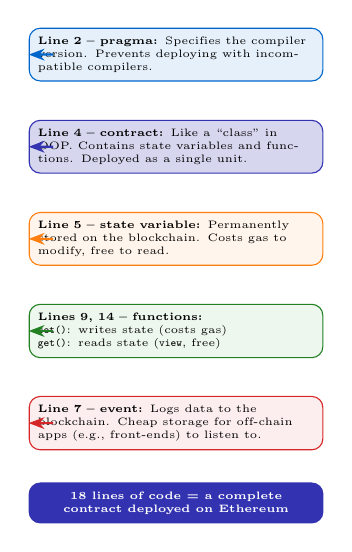
\begin{tikzpicture}[scale=0.78, every node/.style={transform shape}]

% Annotations pointing to code concepts
% Annotation 1: Pragma
\node[draw=mlblue, fill=mlblue!10, rounded corners=4pt, font=\tiny,
      inner sep=4pt, text width=4.5cm, align=left]
      (ann1) at (0,4.5) {\textbf{Line 2 -- pragma:} Specifies the compiler version. Prevents deploying with incompatible compilers.};
\draw[-{Stealth[length=2mm]}, mlblue, thick] (-2.0,4.5) -- (ann1.west);

% Annotation 2: Contract
\node[draw=mlpurple, fill=mllavender4, rounded corners=4pt, font=\tiny,
      inner sep=4pt, text width=4.5cm, align=left]
      (ann2) at (0,3.0) {\textbf{Line 4 -- contract:} Like a ``class'' in OOP. Contains state variables and functions. Deployed as a single unit.};
\draw[-{Stealth[length=2mm]}, mlpurple, thick] (-2.0,3.0) -- (ann2.west);

% Annotation 3: State variable
\node[draw=mlorange, fill=mlorange!8, rounded corners=4pt, font=\tiny,
      inner sep=4pt, text width=4.5cm, align=left]
      (ann3) at (0,1.5) {\textbf{Line 5 -- state variable:} Permanently stored on the blockchain. Costs gas to modify, free to read.};
\draw[-{Stealth[length=2mm]}, mlorange, thick] (-2.0,1.5) -- (ann3.west);

% Annotation 4: Functions
\node[draw=mlgreen!80!black, fill=mlgreen!8, rounded corners=4pt, font=\tiny,
      inner sep=4pt, text width=4.5cm, align=left]
      (ann4) at (0,0.0) {\textbf{Lines 9, 14 -- functions:}\\
      \texttt{set()}: writes state (costs gas)\\
      \texttt{get()}: reads state (\texttt{view}, free)};
\draw[-{Stealth[length=2mm]}, mlgreen!80!black, thick] (-2.0,0.0) -- (ann4.west);

% Annotation 5: Event
\node[draw=mlred, fill=mlred!8, rounded corners=4pt, font=\tiny,
      inner sep=4pt, text width=4.5cm, align=left]
      (ann5) at (0,-1.5) {\textbf{Line 7 -- event:} Logs data to the blockchain. Cheap storage for off-chain apps (e.g., front-ends) to listen to.};
\draw[-{Stealth[length=2mm]}, mlred, thick] (-2.0,-1.5) -- (ann5.west);

% Summary box
\node[draw=mlpurple, fill=mlpurple, text=white, rounded corners=4pt, font=\tiny\bfseries,
      inner sep=4pt, text width=4.5cm, align=center]
      at (0,-2.8) {18 lines of code = a complete\\contract deployed on Ethereum};

\end{tikzpicture}
\end{columns}

\bottomnote{Key insight: Smart contracts are surprisingly concise. This 18-line contract is a fully functional on-chain key-value store. Try it at remix.ethereum.org.}
\end{frame}

% ==================== FRAME 8: DEPLOYING TO ETHEREUM ====================
\begin{frame}{Deploying to Ethereum}
\vspace{-2mm}
\begin{center}
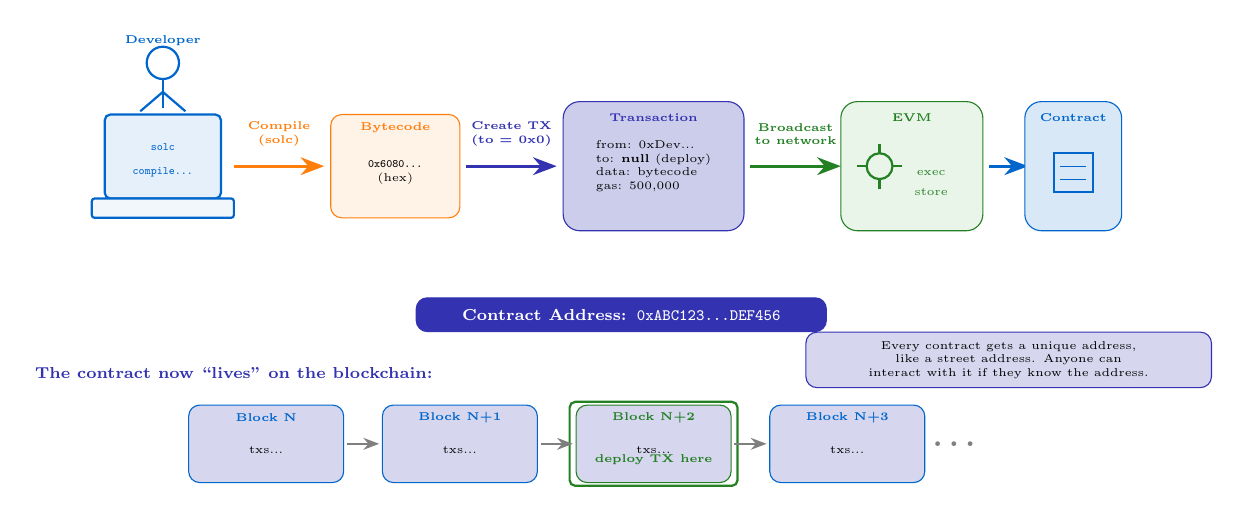
\begin{tikzpicture}[scale=0.82, every node/.style={transform shape}]

% === Developer with laptop ===
% Laptop
\draw[mlblue, thick, fill=mlblue!10, rounded corners=2pt] (-7.0,1.5) rectangle (-5.2,2.8);
\draw[mlblue, thick, fill=mlblue!5, rounded corners=1pt] (-7.2,1.2) rectangle (-5.0,1.5);
% Screen content
\node[font=\tiny, mlblue] at (-6.1,2.3) {\texttt{solc}};
\node[font=\tiny, mlblue] at (-6.1,1.9) {\texttt{compile...}};
% Developer stick figure
\draw[mlblue, thick] (-6.1,3.6) circle (0.25);
\draw[mlblue, thick] (-6.1,3.35) -- (-6.1,2.9);
\draw[mlblue, thick] (-6.1,3.15) -- (-6.45,2.85);
\draw[mlblue, thick] (-6.1,3.15) -- (-5.75,2.85);
\node[font=\tiny\bfseries, mlblue] at (-6.1,3.95) {Developer};

% Arrow: Compile
\draw[-{Stealth[length=3mm]}, mlorange, very thick] (-5.0,2.0) -- (-3.6,2.0);
\node[font=\tiny\bfseries, mlorange, align=center] at (-4.3,2.5) {Compile\\(solc)};

% === Bytecode box ===
\node[draw=mlorange, fill=mlorange!10, rounded corners=4pt, minimum width=2.0cm,
      minimum height=1.6cm, inner sep=3pt] (bytecode) at (-2.5,2.0) {};
\node[font=\tiny\bfseries, mlorange] at (-2.5,2.6) {Bytecode};
\node[font=\tiny, align=center] at (-2.5,1.9) {\texttt{0x6080...}\\(hex)};

% Arrow: Create TX
\draw[-{Stealth[length=3mm]}, mlpurple, very thick] (-1.4,2.0) -- (0.0,2.0);
\node[font=\tiny\bfseries, mlpurple, align=center] at (-0.7,2.5) {Create TX\\(to = 0x0)};

% === Transaction envelope ===
\node[draw=mlpurple, fill=mllavender3, rounded corners=6pt, minimum width=2.8cm,
      minimum height=2.0cm, inner sep=3pt] (tx) at (1.5,2.0) {};
\node[font=\tiny\bfseries, mlpurple] at (1.5,2.75) {Transaction};
\node[font=\tiny, align=left] at (1.5,2.0) {from: 0xDev...\\to: \textbf{null} (deploy)\\data: bytecode\\gas: 500,000};

% Arrow: Submit to network
\draw[-{Stealth[length=3mm]}, mlgreen!80!black, very thick] (3.0,2.0) -- (4.4,2.0);
\node[font=\tiny\bfseries, mlgreen!80!black, align=center] at (3.7,2.5) {Broadcast\\to network};

% === EVM Processing ===
\node[draw=mlgreen!80!black, fill=mlgreen!10, rounded corners=6pt, minimum width=2.2cm,
      minimum height=2.0cm, inner sep=3pt] (evm) at (5.5,2.0) {};
\node[font=\tiny\bfseries, mlgreen!80!black] at (5.5,2.75) {EVM};
% Processing animation
\draw[mlgreen!80!black, thick] (5.0,2.0) circle (0.2);
\foreach \angle in {0,90,180,270} {
    \draw[mlgreen!80!black, thick] ($(5.0,2.0)+(\angle:0.2)$) -- ($(5.0,2.0)+(\angle:0.35)$);
}
\node[font=\tiny, mlgreen!80!black] at (5.8,1.9) {exec};
\node[font=\tiny, mlgreen!80!black] at (5.8,1.6) {store};

% Arrow: Contract created
\draw[-{Stealth[length=3mm]}, mlblue, very thick] (6.7,2.0) -- (7.3,2.0);

% === Contract at address ===
\node[draw=mlblue, fill=mlblue!15, rounded corners=6pt, minimum width=1.5cm,
      minimum height=2.0cm, inner sep=3pt] (contract) at (8.0,2.0) {};
\node[font=\tiny\bfseries, mlblue] at (8.0,2.75) {Contract};
% Contract icon
\draw[mlblue, thick] (7.7,1.6) rectangle (8.3,2.2);
\draw[mlblue, thin] (7.8,2.0) -- (8.2,2.0);
\draw[mlblue, thin] (7.8,1.8) -- (8.2,1.8);

% === Contract address box (below) ===
\node[draw=mlpurple, fill=mlpurple, text=white, rounded corners=4pt, font=\scriptsize\bfseries,
      inner sep=5pt, text width=6cm, align=center] at (1.0,-0.3)
     {Contract Address: \texttt{0xABC123...DEF456}};

% === Blockchain visual (bottom) ===
\node[font=\scriptsize\bfseries, mlpurple] at (-5.0,-1.2) {The contract now ``lives'' on the blockchain:};

% Chain of blocks
\foreach \i/\x/\col/\label in {1/-4.5/mlblue/Block N, 2/-1.5/mlblue/Block N+1, 3/1.5/mlgreen!80!black/Block N+2, 4/4.5/mlblue/Block N+3} {
    \node[draw=\col, fill=mllavender4, rounded corners=4pt,
          minimum width=2.4cm, minimum height=1.2cm, inner sep=2pt]
          (b\i) at (\x,-2.3) {};
    \node[font=\tiny\bfseries, \col] at (\x,-1.9) {\label};
    \node[font=\tiny] at (\x,-2.4) {txs...};
}

% Highlight deployment block
\node[font=\tiny\bfseries, mlgreen!80!black] at (1.5,-2.55) {deploy TX here};
\draw[mlgreen!80!black, thick, rounded corners=2pt] (0.2,-2.95) rectangle (2.8,-1.65);

% Arrows between blocks
\foreach \i/\j in {1/2, 2/3, 3/4} {
    \pgfmathsetmacro{\xfrom}{-4.5 + (\i-1)*3.0 + 1.25}
    \pgfmathsetmacro{\xto}{-4.5 + \i*3.0 - 1.25}
    \draw[-{Stealth[length=2mm]}, mlgray, thick] (\xfrom,-2.3) -- (\xto,-2.3);
}

% Dots
\node[font=\Large\bfseries, mlgray] at (6.2,-2.3) {\ldots};

% Analogy note
\node[draw=mlpurple, fill=mllavender4, rounded corners=4pt, font=\tiny,
      inner sep=4pt, text width=6cm, align=center] at (7.0,-1.0)
     {Every contract gets a unique address,\\like a street address. Anyone can\\interact with it if they know the address.};

\end{tikzpicture}
\end{center}

\bottomnote{Key insight: Deploying is a special transaction with no recipient (to=null). The EVM executes the constructor, stores the bytecode, and assigns a permanent address.}
\end{frame}

% ==================== FRAME 9: REAL-WORLD USE CASES ====================
\begin{frame}{Real-World Use Cases}
\vspace{-2mm}
\begin{center}
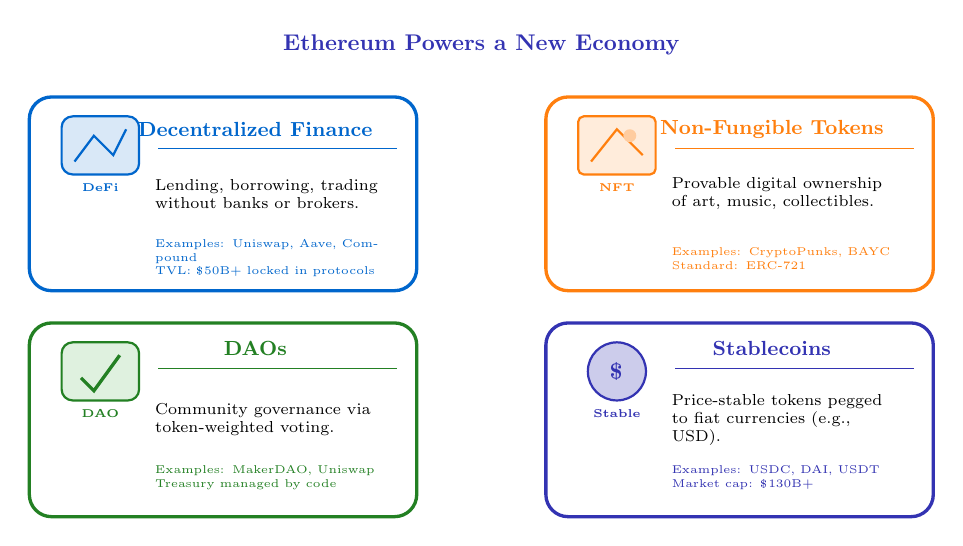
\begin{tikzpicture}[scale=0.82, every node/.style={transform shape}]

\node[font=\normalsize\bfseries, mlpurple] at (0,3.8) {Ethereum Powers a New Economy};

% === Card 1: DeFi (top-left) ===
\node[draw=mlblue, fill=white, rounded corners=8pt, minimum width=6.0cm,
      minimum height=3.0cm, inner sep=5pt] (defi) at (-4.0,1.5) {};
\draw[mlblue, very thick, rounded corners=8pt] (-7.0,0.0) rectangle (-1.0,3.0);

% DeFi icon area
\draw[mlblue, thick, fill=mlblue!15, rounded corners=4pt] (-6.5,1.8) rectangle (-5.3,2.7);
% Chart lines inside
\draw[mlblue, thick] (-6.3,2.0) -- (-6.0,2.4) -- (-5.7,2.1) -- (-5.5,2.5);
\node[font=\tiny\bfseries, mlblue] at (-5.9,1.6) {DeFi};

% DeFi text
\node[font=\small\bfseries, mlblue] at (-3.5,2.5) {Decentralized Finance};
\draw[mlblue, thin] (-5.0,2.2) -- (-1.3,2.2);
\node[font=\scriptsize, text width=3.5cm, align=left] at (-3.3,1.5)
     {Lending, borrowing, trading\\without banks or brokers.};
\node[font=\tiny, mlblue, text width=3.5cm, align=left] at (-3.3,0.5)
     {Examples: Uniswap, Aave, Compound\\TVL: \$50B+ locked in protocols};

% === Card 2: NFTs (top-right) ===
\node[draw=mlorange, fill=white, rounded corners=8pt, minimum width=6.0cm,
      minimum height=3.0cm, inner sep=5pt] (nft) at (4.0,1.5) {};
\draw[mlorange, very thick, rounded corners=8pt] (1.0,0.0) rectangle (7.0,3.0);

% NFT icon area (picture frame)
\draw[mlorange, thick, fill=mlorange!15, rounded corners=2pt] (1.5,1.8) rectangle (2.7,2.7);
% Art inside frame
\draw[mlorange, thick] (1.7,2.0) -- (2.1,2.5) -- (2.5,2.1);
\fill[mlorange!40] (2.3,2.4) circle (0.1);
\node[font=\tiny\bfseries, mlorange] at (2.1,1.6) {NFT};

% NFT text
\node[font=\small\bfseries, mlorange] at (4.5,2.5) {Non-Fungible Tokens};
\draw[mlorange, thin] (3.0,2.2) -- (6.7,2.2);
\node[font=\scriptsize, text width=3.5cm, align=left] at (4.7,1.5)
     {Provable digital ownership\\of art, music, collectibles.};
\node[font=\tiny, mlorange, text width=3.5cm, align=left] at (4.7,0.5)
     {Examples: CryptoPunks, BAYC\\Standard: ERC-721};

% === Card 3: DAOs (bottom-left) ===
\node[draw=mlgreen!80!black, fill=white, rounded corners=8pt, minimum width=6.0cm,
      minimum height=3.0cm, inner sep=5pt] (dao) at (-4.0,-2.0) {};
\draw[mlgreen!80!black, very thick, rounded corners=8pt] (-7.0,-3.5) rectangle (-1.0,-0.5);

% DAO icon area (vote/people)
\draw[mlgreen!80!black, thick, fill=mlgreen!15, rounded corners=4pt] (-6.5,-1.7) rectangle (-5.3,-0.8);
% Vote checkmark
\draw[mlgreen!80!black, very thick] (-6.2,-1.35) -- (-6.0,-1.55) -- (-5.6,-1.0);
\node[font=\tiny\bfseries, mlgreen!80!black] at (-5.9,-1.9) {DAO};

% DAO text
\node[font=\small\bfseries, mlgreen!80!black] at (-3.5,-0.9) {DAOs};
\draw[mlgreen!80!black, thin] (-5.0,-1.2) -- (-1.3,-1.2);
\node[font=\scriptsize, text width=3.5cm, align=left] at (-3.3,-2.0)
     {Community governance via\\token-weighted voting.};
\node[font=\tiny, mlgreen!80!black, text width=3.5cm, align=left] at (-3.3,-2.9)
     {Examples: MakerDAO, Uniswap\\Treasury managed by code};

% === Card 4: Stablecoins (bottom-right) ===
\node[draw=mlpurple, fill=white, rounded corners=8pt, minimum width=6.0cm,
      minimum height=3.0cm, inner sep=5pt] (stable) at (4.0,-2.0) {};
\draw[mlpurple, very thick, rounded corners=8pt] (1.0,-3.5) rectangle (7.0,-0.5);

% Stablecoin icon area (dollar in circle)
\draw[mlpurple, thick, fill=mllavender3] (2.1,-1.25) circle (0.45);
\node[font=\normalsize\bfseries, mlpurple] at (2.1,-1.25) {\$};
\node[font=\tiny\bfseries, mlpurple] at (2.1,-1.9) {Stable};

% Stablecoin text
\node[font=\small\bfseries, mlpurple] at (4.5,-0.9) {Stablecoins};
\draw[mlpurple, thin] (3.0,-1.2) -- (6.7,-1.2);
\node[font=\scriptsize, text width=3.5cm, align=left] at (4.7,-2.0)
     {Price-stable tokens pegged\\to fiat currencies (e.g., USD).};
\node[font=\tiny, mlpurple, text width=3.5cm, align=left] at (4.7,-2.9)
     {Examples: USDC, DAI, USDT\\Market cap: \$130B+};

\end{tikzpicture}
\end{center}

\bottomnote{Key insight: Ethereum's programmability enables entire financial systems to run autonomously as code. DeFi alone processes billions in daily volume.}
\end{frame}

% ==================== FRAME 10: TAKEAWAYS & WHAT'S NEXT ====================
\begin{frame}{Takeaways \& What's Next}
\vspace{-2mm}
\begin{columns}[T]
\column{0.48\textwidth}
\begin{block}{\small Key Principles}
\begin{itemize}\small
    \item $\checkmark$ Ethereum = programmable blockchain
    \item $\checkmark$ Gas prevents abuse and pays validators
    \item $\checkmark$ Smart contracts are self-executing code
    \item $\checkmark$ Once deployed, contracts are (mostly) immutable
    \item $\checkmark$ Real-world impact: DeFi, NFTs, DAOs
\end{itemize}
\end{block}

\vspace{2mm}
\begin{block}{\small The Ethereum Stack}
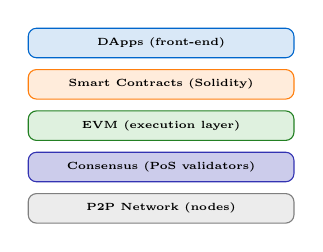
\begin{tikzpicture}[scale=0.75, every node/.style={transform shape}]
  % Stack layers
  \node[draw=mlblue, fill=mlblue!15, rounded corners=3pt, minimum width=4.5cm,
        minimum height=0.5cm, font=\tiny\bfseries] at (0,2.0) {DApps (front-end)};
  \node[draw=mlorange, fill=mlorange!15, rounded corners=3pt, minimum width=4.5cm,
        minimum height=0.5cm, font=\tiny\bfseries] at (0,1.3) {Smart Contracts (Solidity)};
  \node[draw=mlgreen!80!black, fill=mlgreen!15, rounded corners=3pt, minimum width=4.5cm,
        minimum height=0.5cm, font=\tiny\bfseries] at (0,0.6) {EVM (execution layer)};
  \node[draw=mlpurple, fill=mllavender3, rounded corners=3pt, minimum width=4.5cm,
        minimum height=0.5cm, font=\tiny\bfseries] at (0,-0.1) {Consensus (PoS validators)};
  \node[draw=mlgray, fill=mlgray!15, rounded corners=3pt, minimum width=4.5cm,
        minimum height=0.5cm, font=\tiny\bfseries] at (0,-0.8) {P2P Network (nodes)};
\end{tikzpicture}
\end{block}

\column{0.48\textwidth}
% Mind map
\begin{center}
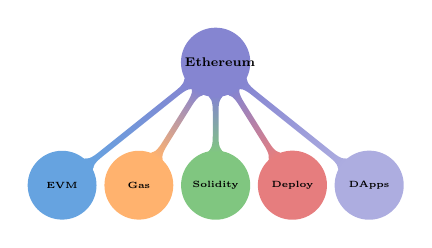
\begin{tikzpicture}[
  scale=0.65,
  every node/.style={transform shape},
  mindmap,
  concept color=mlpurple!60,
  every concept/.append style={minimum size=1.2cm, text width=1.2cm, font=\tiny\bfseries, align=center},
  level 1/.append style={level distance=2.4cm, sibling angle=72},
  level 1 concept/.append style={minimum size=1.0cm, text width=1.0cm}
]
  \node[concept, font=\scriptsize\bfseries] {Ethereum}
    child[concept color=mlblue!60] { node[concept] {EVM} }
    child[concept color=mlorange!60] { node[concept] {Gas} }
    child[concept color=mlgreen!60] { node[concept] {Solidity} }
    child[concept color=mlred!60] { node[concept] {Deploy} }
    child[concept color=mllavender] { node[concept] {DApps} };
\end{tikzpicture}
\end{center}

\vspace{1mm}
\begin{block}{\small What's Next}
\begin{itemize}\scriptsize
    \item ERC-20 tokens: build your own currency
    \item ERC-721: create an NFT collection
    \item DeFi deep dive: AMMs, lending, flash loans
    \item Security: common vulnerabilities and auditing
\end{itemize}
\end{block}
\end{columns}

\vspace{2mm}
\begin{center}

\begin{tikzpicture}
\node[draw=mlpurple, fill=mllavender3, rounded corners=8pt,
      font=\small, inner sep=8pt, text width=13cm, align=center] {%
\textbf{Next lecture: Build your own ERC-20 token!}\\[2pt]
\textit{``In code we trust --- but verify with audits.''}};
\end{tikzpicture}
\end{center}

\bottomnote{Key insight: Ethereum is the foundation of Web3. Understanding smart contracts is essential for anyone working in blockchain, fintech, or decentralized systems.}
\end{frame}

\end{document}
